\begin{figure}
    \centering
\begin{knitrout}
\definecolor{shadecolor}{rgb}{0.969, 0.969, 0.969}\color{fgcolor}
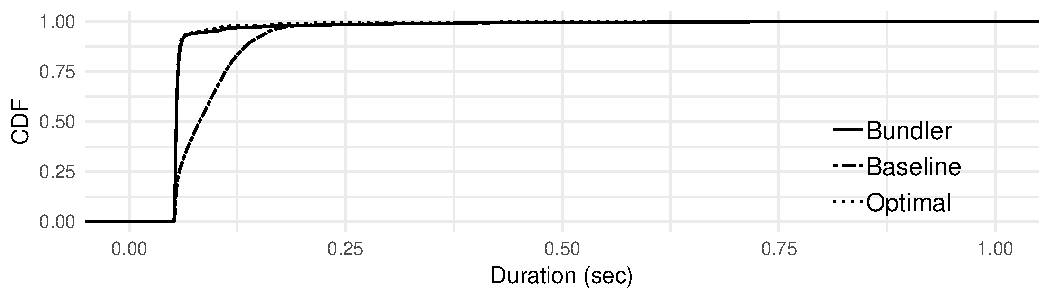
\includegraphics[width=\maxwidth]{figure/eval:best-1} 

\end{knitrout}
    \caption{\name achieves 33\% lower median slowdown. The three graphs show FCT distributions for the indicated request sizes: smaller than 10KB, between 10KB and 1MB, and greater than 1MB.  Note the different y-axis scales for each group of request sizes. For both \name and Optimal, performance benefits come from preventing short flows from queueing behind long ones.}
    \label{fig:eval:best}
\end{figure}
\newcommand{\overviewBenefitsBaselineMedian}{1.62\xspace}
\newcommand{\overviewBenefitsBaselineTail}{10.77\xspace}
\newcommand{\overviewBenefitsBundlerMedian}{1.08\xspace}
\newcommand{\overviewBenefitsBundlerTail}{9.84\xspace}
\newcommand{\overviewBenefitsOptimalMedian}{1.08\xspace}
\newcommand{\overviewBenefitsOptimalTail}{4.46\xspace}
\newcommand{\overviewBenefitsBundlerMedianImprovement}{33\%\xspace}
